\documentclass{beamer}
\usepackage{graphicx}
\usepackage{sourcecodepro}
\usepackage{listings}
\usepackage{amsfonts}
\usepackage{amsmath}
\usepackage{tikz}
\usepackage{tikz-qtree}

\lstset{basicstyle=\ttfamily,breaklines=true}
\usepackage{upquote}
%\def\backtick{\char18}
\lstdefinestyle{backtickstyle}{literate={`}{\char}1, escapechar=@}

\lstdefinelanguage{Kotlin}{
comment=[l]{//},
commentstyle={\color{gray}\ttfamily},
%emph={delegate, filter, first, firstOrNull, forEach, map, mapNotNull, println, return@},
emphstyle={\color{red}},
identifierstyle=\color{black},
keywords={abstract, actual, as, as?, break, by, class, companion, continue, data, do, dynamic, else, enum, expect, false, final, for, fun, get, if, import, in, infix, interface, internal, is, null, object, open, operator, override, package, private, public, return, sealed, set, super, suspend, this, throw, true, try, typealias, val, var, vararg, when, where, while},
keywordstyle={\color{blue}\bfseries},
morecomment=[s]{/*}{*/},
morestring=[b]",
morestring=[s]{"""*}{*"""},
ndkeywords={@Deprecated, @JvmField, @JvmName, @JvmOverloads, @JvmStatic, @JvmSynthetic, Array, Byte, Double, DoublePrecision, Float, Int, Integer, Iterable, Long, Number, Runnable, Short, String},
ndkeywordstyle={\color{Orange}\bfseries},
sensitive=true,
stringstyle={\color{green}\ttfamily},
showstringspaces=false,
}

% Comparison Table
\usepackage{booktabs}
\usepackage{pifont}
\usepackage{float}
\newcommand{\wmark}{\textcolor{orange}{\ding{45}}}
\newcommand{\cmark}{\textcolor{green!80!black}{\ding{51}}}
\newcommand{\xmark}{\textcolor{red}{\ding{55}}}
\newcommand{\mediumwell}[1]{\textcolor{green}{#1}}
\newcommand{\medium}[1]{\textcolor{yellow}{#1}}
\newcommand{\mediumrare}[1]{\textcolor{orange}{#1}}
\newcommand{\rare}[1]{\textcolor{red}{#1}}

\mode<presentation> { \usetheme{Madrid} }

\title{Kotlin\texorpdfstring{$\nabla$}{}}
\subtitle{A Shape Safe eDSL for Differentiable Functional Programming}
\author{Breandan Considine}
\institute[UdeM]{
Universit\'e de Montr\'eal \\
\medskip
\textit{breandan.considine@umontreal.ca}
}
\date{\today}

\begin{document}
    \begin{frame}
        \titlepage
    \end{frame}

    \begin{frame}
        \frametitle{Overview}
        \tableofcontents
    \end{frame}

    \section{A Short Lesson on Computing Derivatives}

    %------------------------------------------------------------------------------------------------

    \begin{frame}
        \frametitle{Differentiation}
        If we have a function, $P(x): \mathbb{R}\rightarrow\mathbb{R}$, recall the derivative is defined as:
        %
        \begin{equation}
            P'(x) = \lim _{h\to 0}{\frac {f(x+h)-f(x)}{h}} = \frac{\Delta y}{\Delta x} = \frac{dP}{dx}
        \end{equation}
        %
        For $P(x_1, \dots, x_n): \mathbb{R}^n\rightarrow\mathbb{R}$, the gradient is a vector of derivatives:
        %
        \begin{equation}
            \nabla P = \left[\frac{\partial P}{\partial x_1}, \dots, \dfrac{\partial P}{\partial x_n}\right]\text{ where }\frac{\partial P}{\partial x_i} = \frac{dP}{dx_i}
        \end{equation}
        %
        For $\mathbf{P}(\mathbf{x}): \mathbb{R}^n\rightarrow\mathbb{R}^m$, the Jacobian is a vector of gradients:
        %
        \begin{equation}
            \mathbf{J}_\mathbf{P} = \left[\nabla P_1, \dots, \nabla P_n \right] \text{ or equivalently, } \mathbf{J}_{ij} = \frac{\partial P_i}{\partial x_j}
        \end{equation}
    \end{frame}

    %------------------------------------------------------------------------------------------------

    \section{Introduction and motivation}

    \begin{frame}
        \frametitle{Automatic differentiation}
        Suppose we have a scalar function $P_k: \mathbb{R}\rightarrow\mathbb{R}$ such that:
        %
        \begin{align*}
            P_k(x) = \begin{cases} p_1(x) = x &\text{if } k=1\\ (p_k\circ P_{k-1})(x)&\text{if } k > 1 \end{cases}
        \end{align*}
        %
        From the chain rule of calculus, we know that:
        %
        \begin{align*}
            \frac{dP}{dp_1} = \frac{dp_k}{dp_{k-1}}\frac{dp_{k-1}}{dp_{k-2}}\dots\frac{dp_2}{dp_1}= {\displaystyle \prod_{i=1}^{k-1} \frac{dp_{i+1}}{dp_{i}}}
        \end{align*}
        %
        For a vector function $\mathbf{P}_k(\mathbf{x}): \mathbb{R}^n\rightarrow\mathbb{R}^m$, the chain rule still applies:
        %
        \begin{align*}
            \mathbf{J}_\mathbf{P_k} = \displaystyle \prod_{i=1}^{k} \mathbf{J}_{p_i} = \underbrace{\bigg(\Big((\mathbf{J}_{p_k} \mathbf{J}_{p_{k-1}}) \dots \mathbf{J}_{p_2}\Big) \mathbf{J}_{p_1}\bigg)}_{\textit{``Reverse accumulation''}} = \underbrace{\bigg(\mathbf{J}_{p_k} \Big(\mathbf{J}_{p_{k-1}} \dots (\mathbf{J}_{p_2} \mathbf{J}_{p_1})\Big)\bigg)}_{\textit{``Forward accumulation''}}
        \end{align*}
        %
        If $\mathbf{P}_{k}$ were a program, what would the type signature of $\mathbf{p}_{0<i<k}$ be?
        %
        \begin{align*}
            \mathbf{p}_i: \mathcal{T}_{out}(\mathbf{p}_{i-1}) \rightarrow \mathcal{T}_{in}(\mathbf{p}_{i+1})
        \end{align*}
        %
    \end{frame}

    %------------------------------------------------------------------------------------------------

    \begin{frame}
        \frametitle{Parameter learning and gradient descent}
        For parametric models, let us rewrite $\mathbf{P}_k(\mathbf{x})$ as:
        %
        \begin{align*}
            \mathbf{\hat P}_k(\mathbf{x}; \mathbf{\boldsymbol\Theta}) = \begin{cases} \mathbf{p}_1(\boldsymbol\theta_1)(\mathbf{x}) &\text{if } k=1\\ \big(\mathbf{p}_k(\boldsymbol\theta_k)\circ \mathbf{\hat P}_{k-1}(\boldsymbol\Theta_{[1, k-1]})\big)\big(\mathbf{x}\big)&\text{if } k > 1 \end{cases} \\
        \end{align*}
        %
        Where $\boldsymbol\Theta = \{\boldsymbol\theta_1, \dots, \boldsymbol\theta_k\}$ are free parameters and $\mathbf{x} \in \mathbb{R}^n$ is a single input. Given $\mathbf{Y} = \{\mathbf{y}^{(1)} = \mathbf{P}(\mathbf{x}^{(1)}), \dots, \mathbf{y}^{(z)} = \mathbf{P}(\mathbf{x}^{(z)})\}$ from an oracle, in order to approximate $\mathbf{P}(\mathbf x)$, repeat the following procedure until $\boldsymbol\Theta$ converges:
        %
        \begin{align*}
            \boldsymbol\Theta \leftarrow \boldsymbol\Theta - \frac{1}{z}\nabla_{\boldsymbol\Theta} \sum_{i=0}^z\mathcal{L}\big(\mathbf{\hat P}_k(\mathbf{x}^{(i)}), \mathbf{y}^{(i)}\big)
        \end{align*}
        %
        If $\mathbf{\hat P}_{k}$ were a program, what would the type signature of $\mathbf{p}_{0<i<k}$ be?
        %
        \begin{align*}
            \mathbf{p}_i: \mathcal{T}_{out}(\mathbf{p}_{i-1}) \times \mathcal{T}(\boldsymbol\theta_{i}) \rightarrow \mathcal{T}_{in}\big(\mathbf{p}_{i+1}(\boldsymbol\theta_{i+1})\big)
        \end{align*}
        %
    \end{frame}

    %------------------------------------------------------------------------------------------------

    \begin{frame}
        \frametitle{Shape checking and inference}
        \begin{itemize}
            \item Scalar functions implicitly represent shape as arity $f(1, 2): \mathbb{R}^2 \rightarrow \mathbb{R}$
            \item To check array programs, we need a type-level encoding of shape
            \item Arbitrary ops (e.g.\ convolution, vectorization) require dependent types
            \item But parametric polymorphism will suffice for many tensor functions
            \item For most algebraic operations, we just need to check for equality\ldots
        \end{itemize}
        {\scriptsize
            \begin{table}
            \begin{tabular}{|c|c|c|c|l|}\hline\multicolumn{1}{|c|}
            {\textbf{Math}}             & \textbf{Derivative}                    & \textbf{Code}                                                                                  &  \textbf{Type Signature}                                                                                                                                                                                    \\ \hline
                $a(b)$                  & $\mathbf{J}_a\mathbf{J}_b$             & \texttt{a(b)}                                                                                  &  $ (\texttt{a}: \mathbb{R}^{\tau}\rightarrow\mathbb{R}^{\pi}, \texttt{b}: \mathbb{R}^{\lambda}\rightarrow\mathbb{R}^{\tau})   \rightarrow (\mathbb{R}^{\lambda}\rightarrow\mathbb{R}^{\pi})$                \\ \hline
                $a + b$                 & $\mathbf{J}_a + \mathbf{J}_b$          & \begin{tabular}{@{}c@{}}\texttt{a + b}\\\texttt{a.plus(b)}\\\texttt{plus(a, b)}\end{tabular}   &  $ (\texttt{a}:  \mathbb{R}^{\tau}\rightarrow\mathbb{R}^{\pi}, \texttt{b}: \mathbb{R}^{\lambda} \rightarrow \mathbb{R}^{\pi}) \rightarrow (\mathbb{R}^{?}\rightarrow \mathbb{R}^{\pi})$                     \\ \hline
                $a   b$                 & $\mathbf{J}_a b + \mathbf{J}_b a$      & \begin{tabular}{@{}c@{}}\texttt{a * b}\\\texttt{a.times(b)}\\\texttt{times(a, b)}\end{tabular} &  $ (\texttt{a}: \mathbb{R}^{\tau}\rightarrow\mathbb{R}^{m \times n}, \texttt{b}: \mathbb{R}^{\lambda}\rightarrow\mathbb{R}^{n \times p})    \rightarrow (\mathbb{R}^{?}\rightarrow\mathbb{R}^{m \times p})$ \\ \hline
                $a ^ b$                 & \tiny{$a^b(a'\frac{b}{a} + b'\ln a)$}  & \begin{tabular}{@{}c@{}}\texttt{a.pow(b)}\\\texttt{pow(a, b)}\end{tabular}                     &  $ (\texttt{a}: \mathbb{R}^{\tau}\rightarrow\mathbb{R}, \texttt{b}: \mathbb{R}^{\lambda}\rightarrow\mathbb{R}) \rightarrow (\mathbb{R}^{?}\rightarrow\mathbb{R}) $                                          \\ \hline
            \end{tabular}
            \end{table}
        }
    \end{frame}

    %------------------------------------------------------------------------------------------------

    \begin{frame}
        \frametitle{Numerical tower}
        \begin{itemize}
            \item Abstract algebra can be useful when generalizing to new structures
            \item Helps us to easily translate between mathematics and source code
            \item Fields are a useful concept when computing over real numbers
            \begin{itemize}
                \item A field is a set $\mathbb{F}$ with two operations $+$ and $\times$, with the properties:
                \begin{itemize}
                    \item Associativity: $\forall a, b, c \in \mathbb{F}, a + (b + c) = (a + b) + c$
                    \item Commutivity: $\forall a, b \in \mathbb{F}, a + b = b + a$ and $a\times b = b\times a$
                    \item Distributivity: $\forall a, b, c \in \mathbb{F}, a \times (b \times c) = (a \times b) \times c$
                    \item Identity: $\forall a \in \mathbb{F}, \exists 0$, $ 1 \in F$ s.t. $a + 0 = a$ and $a\times 1= a$
                    \item $+$ inverse: $\forall a\in \mathbb{F}, \exists (-a)$ s.t. $a + (-a) = 0$
                    \item $\times$ inverse: $\forall a\neq 0 \in \mathbb{F}, \exists (a^{-1})$ s.t. $a \times a^{-1} = 1$
                \end{itemize}
            \end{itemize}
            \item Extensible to other number systems (e.g.\ complex, dual numbers)
            \item What is a program, but a series of arithmetic operations?
        \end{itemize}
    \end{frame}

    %------------------------------------------------------------------------------------------------

    \begin{frame}
        \frametitle{Why Kotlin?}
        \begin{itemize}
            \item Goal: To implement automatic differentiation in Kotlin
            \item Kotlin is a language with strong static typing and null safety
            \item Supports first-class functions, higher order functions and lambdas
            \item Has support for algebraic data types through sealed classes
            \item Extension functions, operator overloading \& other syntax sugar
            \item Offers features for embedding domain specific languages (DSLs)
            \item Access to all libraries and frameworks in the JVM ecosystem
            \item Multi-platform and cross-platform (JVM, Android, iOS, JS, native)
        \end{itemize}
        \begin{center}
            
\includegraphics[scale=0.05]{../figures/kotlin.png}
        \end{center}
    \end{frame}

    \begin{frame}
        \frametitle{Kotlin\texorpdfstring{$\nabla$}{} Priorities}
        \begin{itemize}
            \item Type system
            \begin{itemize}
                \item Strong type system based on algebraic principles
                \item Leverage the compiler for static analysis
                \item No implicit broadcasting or shape coercion
                \item Parameterized numerical types and arbitary-precision
            \end{itemize}
            \item Design principles
            \begin{itemize}
                \item Functional programming and lazy numerical evaluation
                \item Eager algebraic simplification of expression trees
                \item Operator overloading and tapeless reverse mode AD
            \end{itemize}
            \item Usage desiderata
            \begin{itemize}
                \item Generalized AD with functional array programming
                \item Automatic differentiation with infix and Polish notation
                \item Partials and higher order derivatives and gradients
            \end{itemize}
            \item Testing and validation
            \begin{itemize}
                \item Numerical gradient checking and property-based testing
                \item Performance benchmarks and thorough regression testing
            \end{itemize}
        \end{itemize}
    \end{frame}

    \begin{frame}
        \frametitle{Feature Comparison Matrix}
            \begin{center}
            \begin{tabular}{lllllllll}
            \textbf{Framework} & \textbf{Language}  & SD     & AD     & FP     & TS     & SS     & DP     & MP     \\ \hline
            Kotlin$\nabla$     & Kotlin             & \cmark & \cmark & \cmark & \cmark & \cmark & \wmark & \wmark \\
            DiffSharp          & F\#                & \xmark & \cmark & \cmark & \cmark & \xmark & \cmark & \xmark \\
            TensorFlow.FSharp  & F\#                & \xmark & \cmark & \cmark & \cmark & \cmark & \cmark & \xmark \\
            Myia               & Python             & \cmark & \cmark & \cmark & \cmark & \cmark & \cmark & \xmark \\
            Deeplearning.scala & Scala              & \xmark & \cmark & \cmark & \cmark & \xmark & \cmark & \xmark \\
            Nexus              & Scala              & \xmark & \cmark & \cmark & \cmark & \cmark & \cmark & \xmark \\
            Lantern            & Scala              & \xmark & \cmark & \cmark & \cmark & \xmark & \cmark & \xmark \\
            Grenade            & Haskell            & \xmark & \cmark & \cmark & \cmark & \cmark & \xmark & \xmark \\
            Eclipse DL4J       & Java               & \xmark & \cmark & \xmark & \cmark & \xmark & \xmark & \xmark \\
            Halide             & C++                & \xmark & \cmark & \xmark & \cmark & \xmark & \cmark & \xmark \\
            Stalin$\nabla$     & Scheme             & \xmark & \cmark & \cmark & \xmark & \xmark & \xmark & \xmark \\
        \end{tabular}
        \end{center}
        \footnotesize{SD: Symbolic Differentiation, AD: Automatic Differentiation, FP: Functional Program, TS: Type-Safe, SS: Shape Safe, DP: Differentiable Programming, MP: Multiplatform}
    \end{frame}

    \section{Usage}

    \begin{frame}[fragile]
        \frametitle{Usage}
            \squeezeup\begin{figure}[!htb]
                  \begin{center}
                  \begin{tabular}{c}
                  \begin{lstlisting}[language=Kotlin, gobble=22]
                      val z = sin(10 * (x * x + pow(y, 2))) / 10
                  \end{lstlisting}
                  \end{tabular}
                  \end{center}
                  \vspace{10}
                  \squeezeup\centering
                  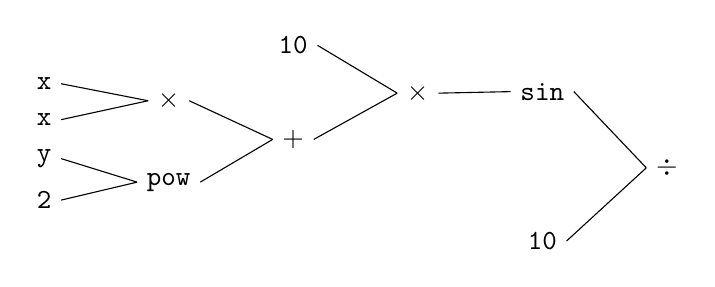
\begin{tikzpicture}[grow=left]
                      \tikzset{level distance=45pt}\squeezeup\squeezeup
                      \Tree [.$\div$ [.\texttt{sin} [.$\times$ \texttt{10} [.$+$ [.$\times$ \texttt{x} \texttt{x} ] [.\texttt{pow} \texttt{y} \texttt{2} ] ] ] ] \texttt{10} ]
                  \end{tikzpicture}
                  \squeezeup\squeezeup\squeezeup\caption{Implicit DFG constructed by the above expression, \texttt{z}.}
    \end{figure}
    \end{frame}

    \section{Architectural Overview}


    \begin{frame}[fragile]
        \frametitle{How do we define algebraic types in Kotlin\texorpdfstring{$\nabla$}{}?}
\begin{center}
\begin{tabular}{c}
        \begin{lstlisting}[language=Kotlin, gobble=12]
            // T: Group<T> is effectively a self type
            interface Group<T: Group<T>> {
                operator fun plus(f: T): T
                operator fun unaryMinus(): X
                operator fun minus(f: X): X = this + -f
                operator fun times(f: T): T
            }

            interface Field<X: Group<X>> {
                val e: X
                val one: X
                val zero: X
                operator fun div(f: X): X = this * f.pow(-one)
                infix fun pow(f: X): X
                fun ln(): X
            }
        \end{lstlisting}
\end{tabular}
\end{center}
    \end{frame}


    \begin{frame}[fragile]
        \frametitle{Algebraic Data Types}
        \begin{lstlisting}[language=Kotlin, gobble=12]
            class Var<X: Fun<X>>(val lbl: String): Fun<X>()
            class Sum<X: Fun<X>>(val f1: X, val f2: X): Fun<X>()
            class Pdt<X: Fun<X>>(val f1: X, val f2: X): Fun<X>()
            class Const<X: Fun<X>>(val num: Number): Fun<X>()

            sealed class Fun<X: Fun<X>>: Field<Fun<X>> {
                open fun diff(): Fun<X> = when(this) {
                    is Const -> Zero
                    is Sum -> f1.diff() + f2.diff()
                    is Pdt -> f1.diff() * f2 + f1 * f2.diff()
                    is Var -> One
                }

                operator fun plus(f: Fun<X>) = Sum(this, f)
                operator fun times(f: Fun<X>) = Pdt(this, f)
            }
        \end{lstlisting}
    \end{frame}

    \begin{frame}[fragile]
        \frametitle{Expression simplification}
        \begin{lstlisting}[language=Kotlin, gobble=12]
            operator fun times(f: Fun<X>): Fun<X> = when {
              // Constant propagation and folding optimizations
              this is Const && num == 0.0 -> Const(0.0)
              this is Const && num == 1.0 -> f
              f is Const && f.num == 0.0 -> exp
              f is Const && f.num == 1.0 -> this
              this is Const && f is Const -> Const(num * f.num)
              // Only instantiate a product node on last resort
              else -> Pdt(this, e)
            }

            // Sum(Pdt(Const(2.0), Var()), Const(6.0))
            val q = Const(2.0) * Sum(Var(), Const(3.0))
        \end{lstlisting}
    \end{frame}


    \begin{frame}[fragile]
        \frametitle{Extension functions and contexts}
\begin{center}
\begin{tabular}{c}
        \begin{lstlisting}[language=Kotlin, gobble=12]
            object DoublePrecision {
                operator fun Number.times(f: Fun<KDouble>) =
                    Const(toDouble()) * f
            }

            class KDouble(num: Double): Const<KDouble>(num) {
                override val e by lazy { KDouble(Math.E) }
                override val one by lazy { KDouble(1.0) }
                override val zero by lazy { KDouble(0.0) }
                // Adapters for wrapping primitive Double...
            }

            // Uses * operator in Double context
            fun Fun<KDouble>.multiplyByTwo() =
                with(DoublePrecision) { 2 * this }
        \end{lstlisting}
\end{tabular}
\end{center}
    \end{frame}


    \begin{frame}[fragile]
        \frametitle{Shape safe vector addition and inference (toy example)}
        \begin{lstlisting}[language=Kotlin, gobble=12, style=backtickstyle]
            interface Nat<T: D0> { val value: Int }
            // Type level integer literals for shape checking
            sealed class D0(open val value: Int = 0)
              { companion object: D0(), Nat<D0> }
            open class D1(override val value: Int = 1): D0(2)
              { companion object: D1(), Nat<D1> }
            open class D2(override val value: Int = 2): D1(2)
              { companion object: D2(), Nat<D2> }

            // <L: D0> accepts 0 <= L via Liskov substitution
            class Vec<E, L: D0>(val len: L, val es: List<E>)
            operator fun <L: D0, V: Vec<Int, L>> V.plus(v: V) =
              Vec<Int, L>(len, es.zip(v.es).map { it.l + it.r })

            val Y= Vec(D2, listOf(1,2)) + Vec(D2, listOf(3,4))
            val X= Vec(D1, listOf(1)) + Y // Compiler error!
        \end{lstlisting}
    \end{frame}

    \begin{frame}[fragile]
        \frametitle{Automatic test case generation}
        \begin{lstlisting}[language=Kotlin, gobble=12]
            val x by Var()
            val y by Var()

            val z = y * (sin(x * y) - x) // Function under test
            val dz_dx = d(z) / d(x)      // Automatic derivative
            val manualDx = y * (cos(x * y) * y - 1)

            "dz/dx should be y * (cos(x * y) * y - 1)" {
                assertAll (DoubleGenerator) { cx, cy ->
                    // Evaluate the results at a given seed
                    val autoEval = dz_dx(x to cx, y to cy)
                    val symbEval = manualDx(x to cx, y to cy)
                    // Only pass iff |adEval - manualEval| < eps
                    autoEval shouldBeApproximately symbEval
                }
            }
        \end{lstlisting}
    \end{frame}

    \section{Plotting}

    \begin{frame}[fragile]
        \frametitle{Usage: Plotting higher derivatives of nested functions}
        \begin{lstlisting}[language=Kotlin, gobble=12]
            // Use double-precision floating point numerics
            with(DoublePrecision) {
              val x = Var()
              val y = sin(sin(sin(x)))/x + x*sin(x) + cos(x) + x

              // Perform lazy symbolic differentiation
              val dy_dx = d(y) / d(x)
              val d2y_dx = d(dy_dx) / d(x)
              val d3y_dx = d(d2y_dx2) / d(x)
              val d4y_dx = d(d3y_dx3) / d(x)
              val d5y_dx = d(d4y_dx4) / d(x)

              plot(-9..9, dy_dx, dy2_dx, d3y_dx, d4y_dx, d5y_dx)
            }
        \end{lstlisting}
    \end{frame}

    \begin{frame}
        \frametitle{$y = \frac{\sin{\sin{\sin{x}}}}{x} + x \sin{x} + \cos{x} + x$, $\frac{dy}{dx}$, $\frac{d^{2}y}{dx^2}$, $\frac{d^{3}y}{dx^3}$, $\frac{d^{4}y}{dx^4}$, $\frac{d^{5}y}{dx^5}$}
        \begin{center}
            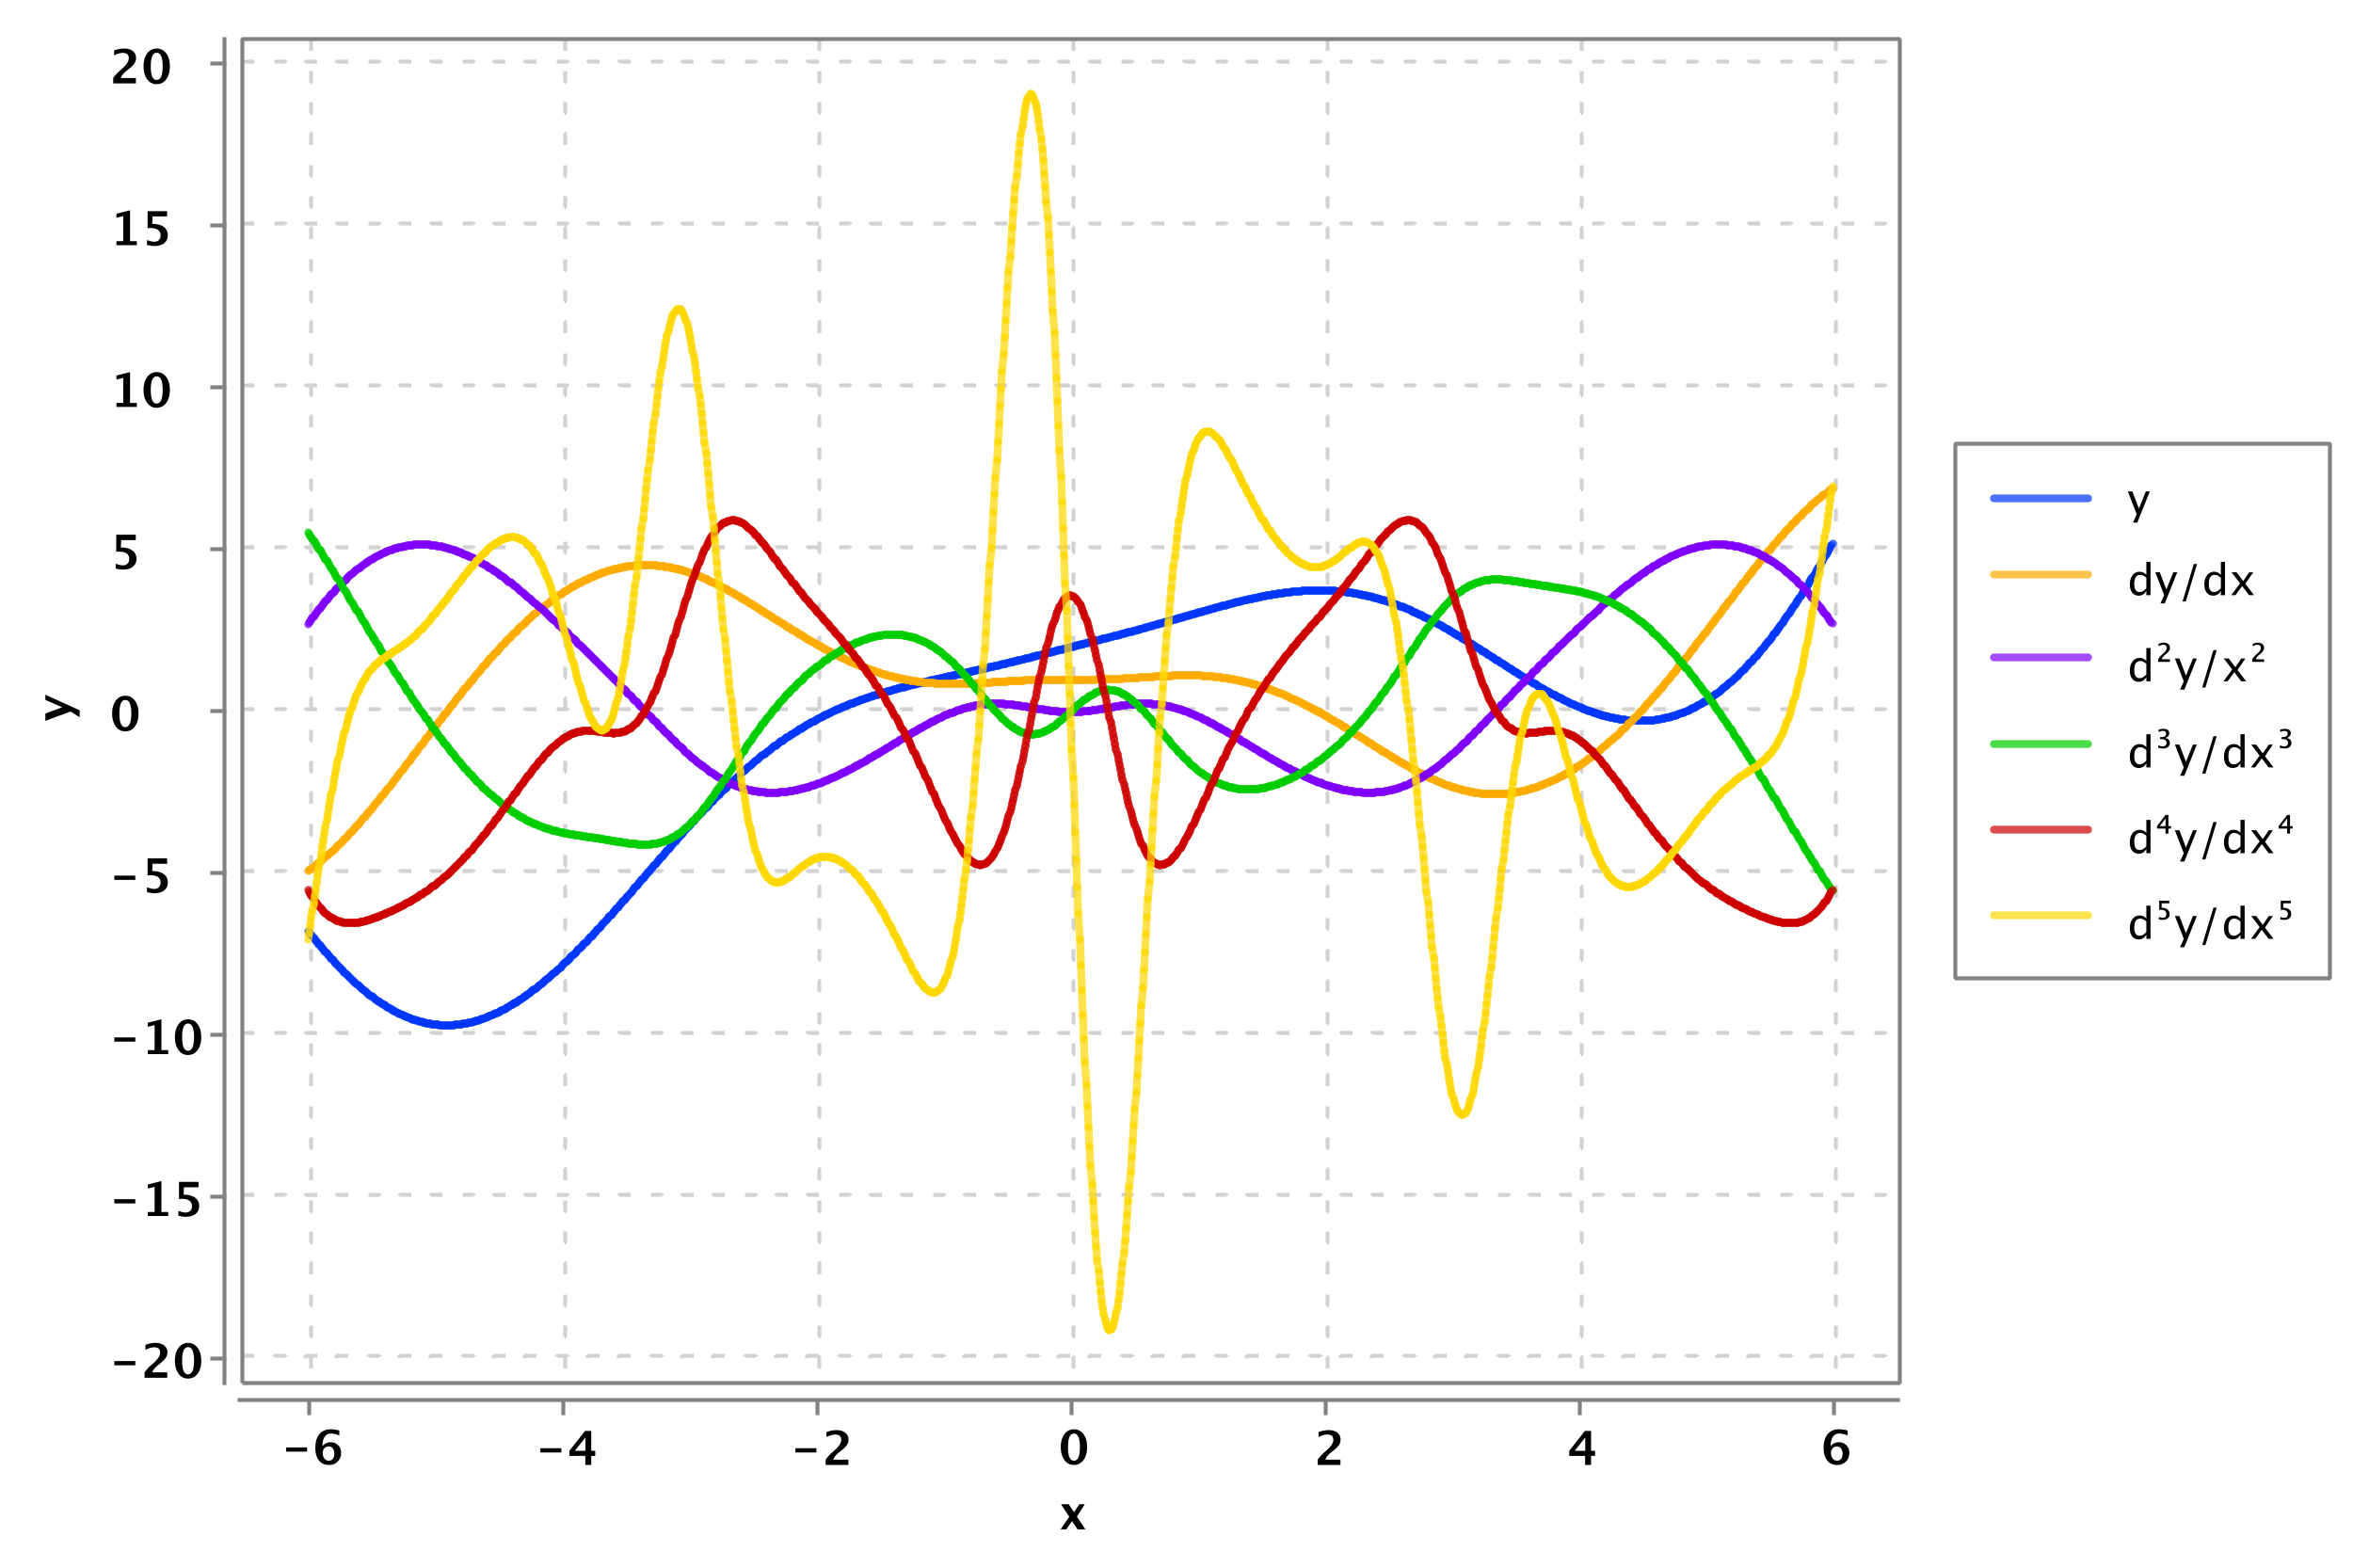
\includegraphics[scale=0.35]{../figures/plot.png}
        \end{center}
    \end{frame}

    \begin{frame}[fragile]
        \frametitle{Usage: 3D plotting with mixed higher order partials}

        \begin{center}
            \begin{tabular}{c}
        \begin{lstlisting}[language=Kotlin, gobble=12]
            with(DoublePrecision) {
                val x = Var()
                val y = Var()

                val z = sin(10 * (x * x + pow(y, 2))) / 10
                val dz_dx = d(z) / d(x)
                val d2f_dxdy = d(dz_dx) / d(y)
                val d3z_d2xdy = d(d(dz_dx) / d(y)) / d(x)

                plot3d(-1, 1, d3z_d2xdy)
            }
        \end{lstlisting}
            \end{tabular}
        \end{center}
    \end{frame}

    \begin{frame}
        \frametitle{$z = \sin(10(x^2 + y^2)) / 10$, $\frac{\partial^3 z}{\partial^2 x \partial y}$}
        \begin{center}
            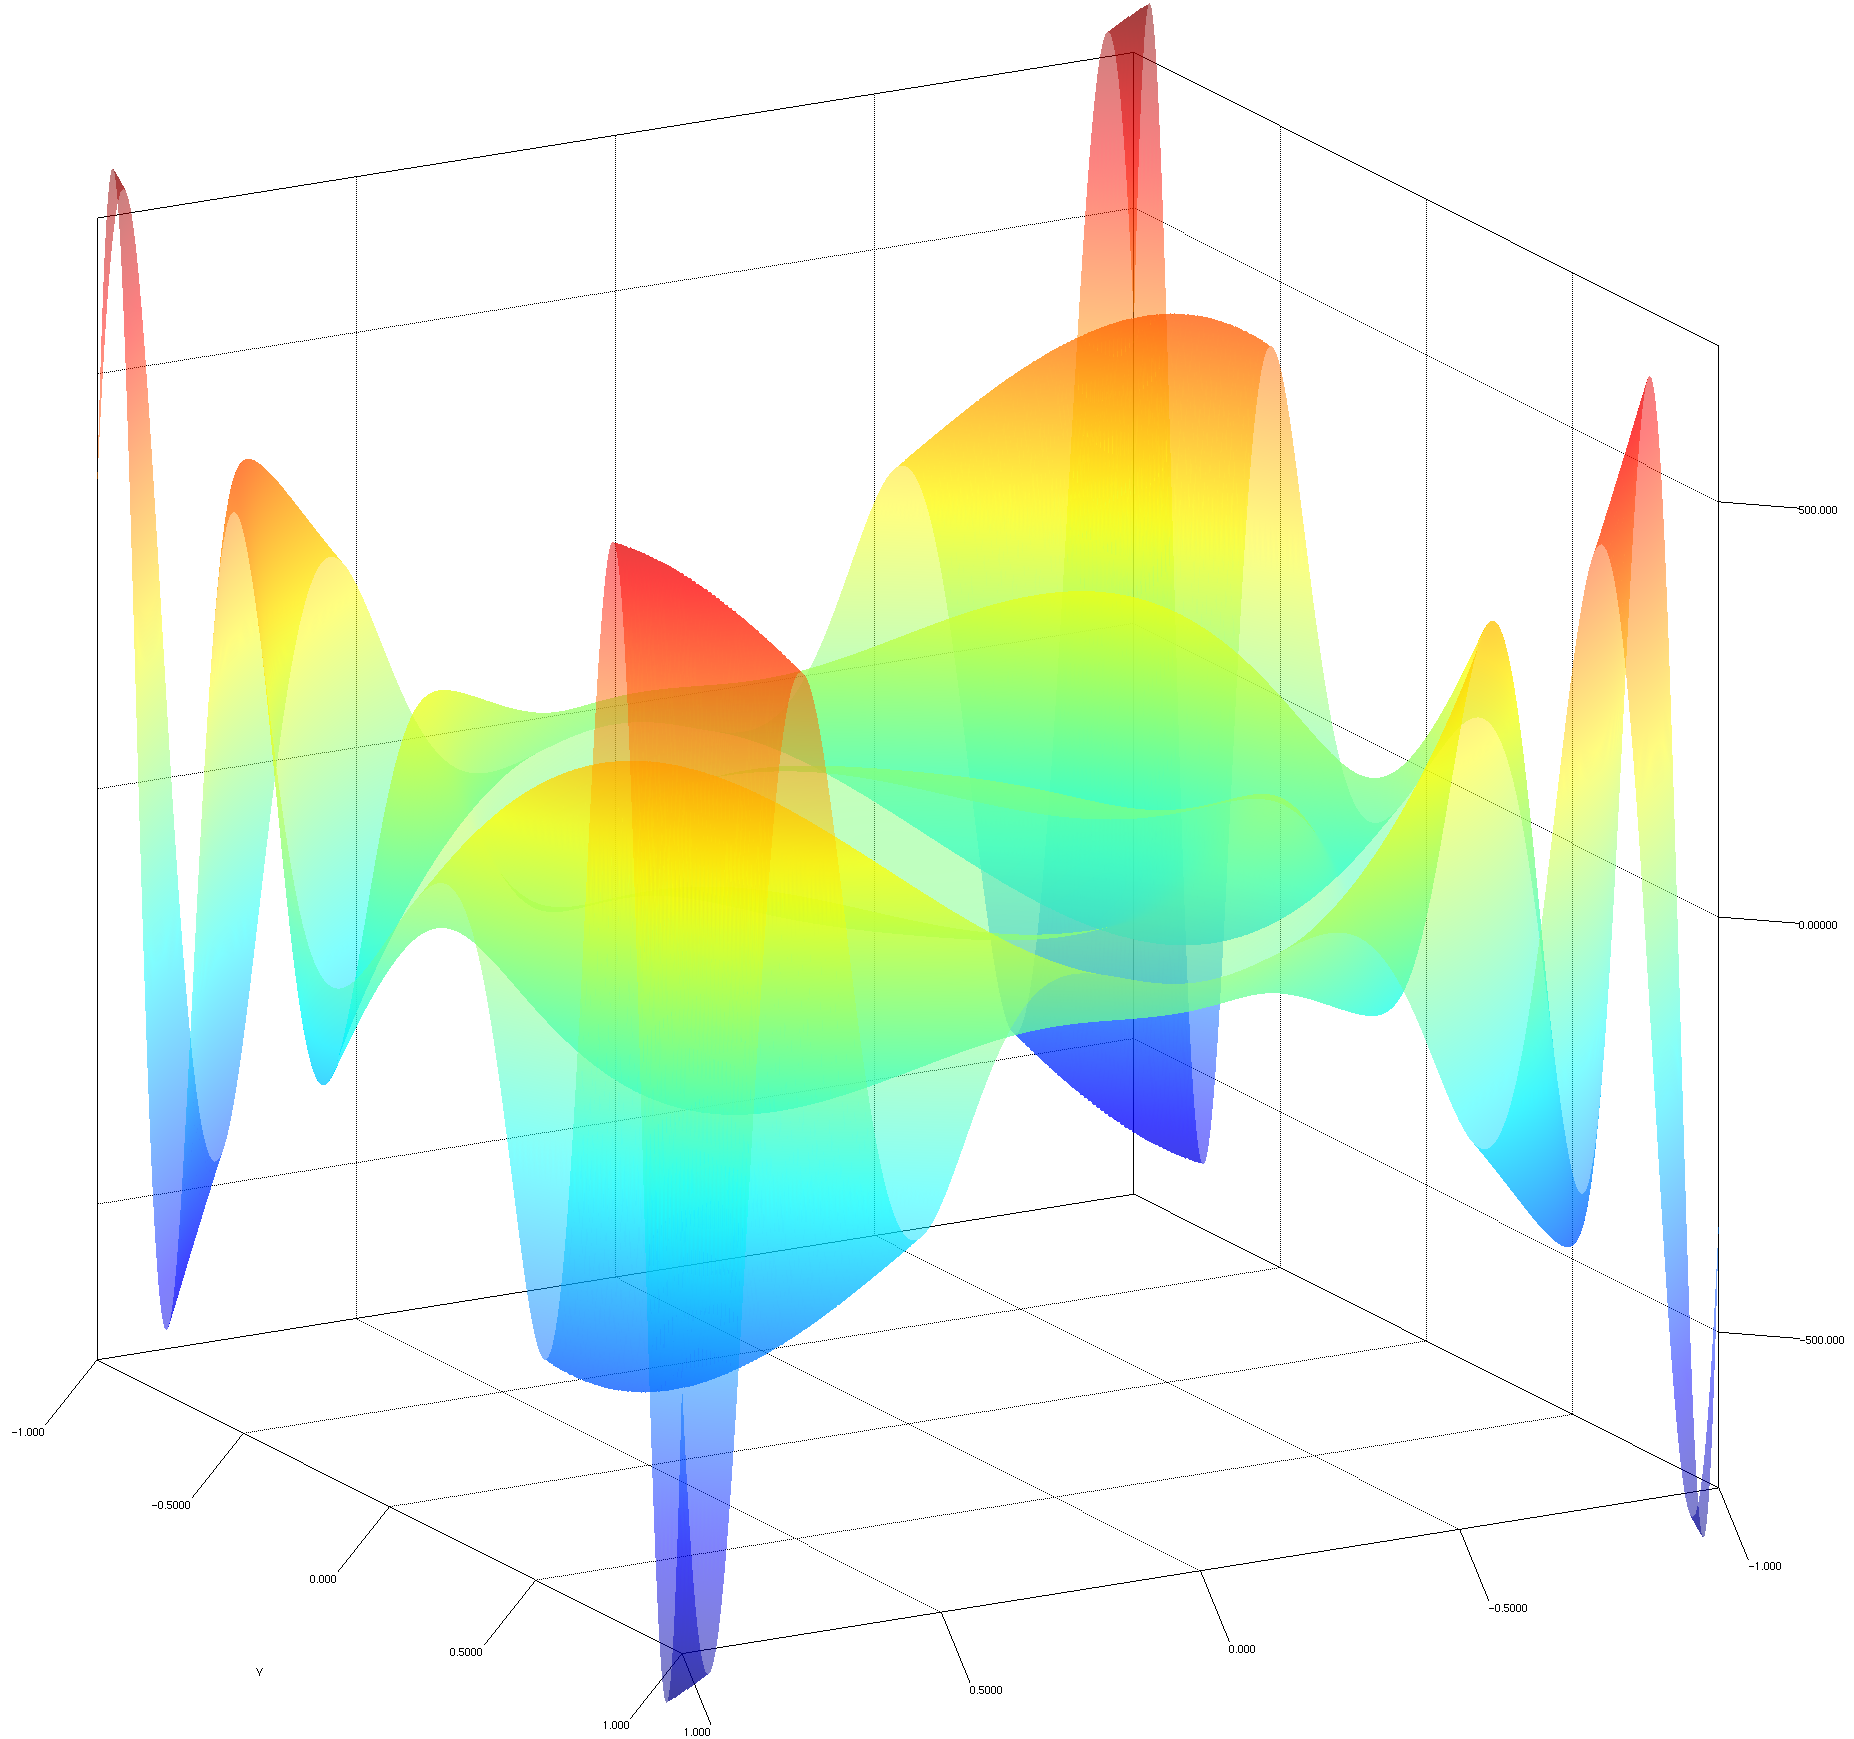
\includegraphics[scale=0.4]{../figures/plot3d.png}
        \end{center}
    \end{frame}

    \section{Future exploration}

    \begin{frame}
        \frametitle{Further directions to explore}
        \begin{itemize}
            \item Theory Directions
            \begin{itemize}
                \item Generalization of types to higher order functions, vector spaces
                \item Dependent types via code generation to type-check convolution
                \item General programming operators and data structures
                \item Imperative define-by-run array programming syntax
                \item Program induction and synthesis, cf.
                \begin{itemize}
                    \item The Derivative of a Regular Type is its Type of One-Hole Contexts
                    \item The Differential Lambda Calculus (2003)
                \end{itemize}
                \item Asynchronous gradient descent (cf. HogWild, YellowFin, et al.)
            \end{itemize}
            \item Implementation Details
            \begin{itemize}
                \item Closer integration with Kotlin/Java standard library
                \item Encode additional structure, i.e. function arity into type system
                \item Vectorized optimizations for matrices with certain properties
                \item Configurable forward and backward AD modes based on dimension
                \item Automatic expression refactoring for numerical stability
                \item \href{https://discuss.kotlinlang.org/t/primitive-type-specialization/11022}{Primitive type specialization}, i.e. \texttt{FloatVector <: Vector<T>}?
            \end{itemize}
        \end{itemize}
    \end{frame}

    \begin{frame}
        \begin{center}
            \Huge{Learn more at: \\~\\
            \url{http://kg.ndan.co}}
        \end{center}
    \end{frame}

    \begin{frame}
        \frametitle{Special thanks}
        \begin{itemize}
            \begin{center}
                \huge{
                Liam Paull \\
                Michalis Famelis \\
                }
                \vspace{10}
                
\includegraphics[scale=0.4]{../figures/cser_logo.png}\\
                \vspace{10}
                
\includegraphics[scale=0.1]{../figures/udem.png}
                
\includegraphics[scale=0.4]{../figures/mila.png}
            \end{center}
        \end{itemize}
    \end{frame}
\end{document}

%------------------------------------------------------------------------------------------------

%    \begin{frame}
%        \frametitle{Symbolic differentiation}
%        \begin{itemize}
%            \item What about evaluating functions symbolically?
%            \item Computer algebra systems for manipulate symbolic formulas
%        \end{itemize}
%    \end{frame}

%------------------------------------------------------------------------------------------------

%    \begin{frame}
%        \frametitle{Automatic differentiation}
%        \begin{itemize}
%            \item Derivatives can be calculated automatically? (Wengert, 1964)
%            \item Code as an \textit{exact} symbolic representation of functions
%            \item To reason about code we need the ability to treat \textit{code as data}:
%            \begin{itemize}
%                \item Reflection and metaprogramming
%                \item Domain specific languages
%                \item First-class functions
%            \end{itemize}
%        \end{itemize}
%    \end{frame}

%------------------------------------------------------------------------------------------------

%    \begin{frame}
%        \frametitle{Differentiable [functional] programming}
%        \begin{itemize}
%            \item What is a program, but a series of arithmetic operations?
%            \item What are arithmetic operations but syntactic sugar for functions?
%            \item Functions can be composed of other functions or chained in sequence
%            \item High school calculus gives us rules for differentiating function chains
%            \item Pearlmutter \& Siskind teach us AD is possible just using FP (2016)
%            \item Wang, Rompf, et al. show us this is possible \textit{without a tape}! (2018)
%        \end{itemize}
%    \end{frame}

%------------------------------------------------------------------------------------------------

%    \begin{frame}
%        \frametitle{Differentiable programming with algebraic types}
%        \begin{itemize}
%            \item Combine the tools from mathematics and CS
%            \item Type safety
%            \item Static analysis
%            \item Allows us to preserve symmetries that are not obvious
%            \item There is an abstract algebra for tensor manipulations
%            \item Can be encoded using OOP and parametric polymorphism
%            \item \href{https://arxiv.org/pdf/1610.07690.pdf}{Operational Calculus for Differentiable Programming}
%        \end{itemize}
%    \end{frame}

%------------------------------------------------------------------------------------------------
